
\chapter{Laban Movement Analysis of Movements Recorded by Kinect, Using Machine Learning}
\label{chap:firstchap}

\section{Laban Movement Analysis (LMA)}
LMA is a well-established and widely accepted systematic language for describing
and documenting movement. LMA's comprehensiveness as a motor analysis method
could be inferred from its diverse use in research: it has been used to evaluate
fighting behaviors of rats \cite{foroud2003development}, to analyze behavior of
nonhuman animals in naturalistic settings \cite{fagan1997observing}, to diagnose
autistic individuals \cite{dott1995aesthetic}, to evaluate motor recovery of
stroke patients \cite{foroud2006changes}, and to characterize the development of
infants' reaching movements \cite{foroud2012consummatory}. In recent years it
gained additional popularity among computer science researchers who have used it
in studies that describe, recognize or create bodily emotional expressions for
applications in human-robot interactions, interactive games such as the Xbox,
and in animations \cite{camurri2003recognizing,rett,
Zacharatos, lourens2010communicating, zhao2005acquiring,masuda2009emotion,
masuda2010motion}, and recently it has even been attempted, through the use of
EEG, to identify the brain mechanisms underlying the production of some of the
LMA motor elements \cite{cruz2014neural}. In addition, some studies have found
correlations between some Laban motor elements and personality traits or
emotional states \cite{levy2003use, shafir2015emotion}.
\par Analyzing movements using LMA is advantageous over other methods, as it
captures various qualitative \textbf{motor elements} (movement characteristics)
in addition to quantitative (kinematic) aspects of the movement. LMA categorizes
movement with four main components: Body, Effort, Shape, and Space.
\textbf{Body} (i.e. which \textit{body parts} move) and \textbf{Space} (i.e. the
direction of movement such as Vertical:
\underline{Up/Down}, Sagittal: \underline{Forward/Back} or Horizontal: to the
side), describe how the many spatial-temporal body and limb relationships
change. The category of Body also
includes specific common \textit{body actions} such as jump and walk.
\textbf{Effort} describes the qualitative aspect of movement expressive of a
person's inner attitude
towards movement via four Effort factors: Weight, Time, Space and Flow. Each
Factor identifies movement on a continuum between two poles: fighting against
the motor quality of that factor and indulging in that quality. 
1) \textbf{\textit{Weight Effort}}, identifies the amount of force or pressure
exerted in movement, on the continuum from \underline{Strong} to \underline{Light} (and
movements lacking weight activation, i.e., \underline{Passive/Heavy} movement); 
2) \textbf{\textit{Time Effort}} identifies the degree of urgency or
acceleration/deceleration involved in a movement, i.e., \underline{Sudden} or
\underline{Sustained} movement; 
3) \textbf{\textit{Space Effort}}, describes the focus or
attitude towards a chosen pathway, i.e., is the movement \underline{Direct} or
\underline{Indirect} and 
4)~ \textbf{\textit{Flow Effort}} describes the element of control or
the degree to which a movement is \underline{Bound}, i.e., controlled by muscle
contraction, versus \underline{Free}, i.e., being released/liberated.
Finally, \textbf{Shape} refers to the way the body 'sculpts' itself in space: It
describes the changes in the relationship of body parts to one another and to
the surrounding environment that occur when a body moves (e.g., whether the body
\underline{Encloses} or \underline{Spreads, Rises} or \underline{Sinks}, etc.).
In addition, LMA examines other movement characteristic, such as the
\textbf{phrasing} of the movement, which means the
way movement elements are sequenced into action. Analogous to phrasing in music,
a motor phrase can be \underline{rhythmic} (repetitive), \underline{even}
(monotonous), etc.
(For a more detailed and systematic description of LMA see
\cite{bartenieff1980body,studd, fernandes2014moving}).
\par As can be seen from this short description, LMA is very thorough. It
captures a variety of movement dimensions, and has therefore become the preferred method
for movement analysis used by many scientists. Indeed, in a recent study that
used both Effort-Shape (part of LMA) and kinematic analyses to identify movement
characteristics associated with positive and negative emotions experienced
during walking, more differences among emotions were identified with
Effort-Shape analysis than with kinematic analysis \cite{gross2012effort} , and
both Chi et al.,\cite{chi2000emote} and Masuda et al.,\cite{masuda2010motion}
chose to develop a computer generated animation \cite{chi2000emote} or robotic
\cite{masuda2010motion}  system that transforms simple movements into
emotionally expressive movements, by modifying certain movement parameters of
the animated character or robot, based on LMA. Thus, we have chosen to use LMA
for the purpose of developing the automated method for recognizing movement
characteristics.
\par Because LMA is a comprehensive system with tens of different motor
characteristics, and because many of the current applications for automated
analysis of movement have to do with creation or recognition of emotional
expressions in movements, we  focused this study on identification of the 18
Laban motor elements (Table \ref{mixedSummary} in the results section)
found to be associated with specific emotions[18]. Thus, we created a data base
of movements captured by a Kinect camera and developed machine learning-based,
algorithms for automated identification of the 18 Laban motor elements
expressive of emotion, from our Kinect data.

\section{Method}
\subsection{Kinect Sensor Data}
The Kinect Software Development Kit (SDK) detects the skeleton of the videotaped
moving person and provides the 3D coordinates of 24 joints along this skeleton,
as seen in Fig. ~\ref{skeleton}.

\begin{figure}[h]
\centering
\includegraphics[width=2.5in]{graphics/Laban/skeleton.jpg}
\caption{Skeleton positions relative to the human body}
\label{skeleton}
\end{figure}

The coordinates of these joints are given in a
“real world” coordinate system whose origin [0,0,0] is in the sensor and whose
x, y, and z axis are as depicted in Fig. \ref{Coordinate} below. Data were
collected by the Kinect camera at 30 Hz.


\begin{figure}[h] \centering
\includegraphics[width=2.5in]{graphics/Laban/KinectV2CoordinateSystem.jpg}
\caption{Kinect Coordinate System}
\label{Coordinate}
\end{figure}

\subsection{Clip collection}
In order to develop the ability to automatically identify Laban motor elements
we had to ensure that the movements in the data set used for the machine
learning, included those elements. Thus, for this study, we generated two
specific data sets:
\begin{itemize}
  \item CMA dataset: This dataset consisted of clips of movements performed by
  Certified (Laban) Movement Analysts experts (CMAs). Six CMAs performed
  movement sequences of approximately 3 seconds long, which consisted of different 
  combinations of LMA motor elements. Before each movement sequence (clip) the
  CMAs were given a list of 2-4 Laban motor elements out of the 18 motor elements that 
  were studied, and were instructed to move any movement that they want, as long 
  as it incorporates those required motor elements. Each of the CMAs moved about 
  80 such different combinations of 2-4 motor elements, for a total of 550 clips. 
  To achieve uniform distribution of the Laban qualities over the dataset, in every 
  movement sequence (clip) each CMA was asked to perform actions that included
  several specific motor elements, and nothing but them.
  \item Non-CMA dataset: This dataset consisted of movement sequences performed
  by two people without a background in LMA, who were asked to move as if they are 
  performing different every-day tasks such as greeting a friend or playing with 
  a balloon. Their movements lasted also about 3 seconds long and a total of 30
  such clips were collected. Their movements were tagged by a CMA who determined 
  which of the 18 Laban qualities that we tested in this study appeared in each of 
  their movement sequences (clips).
\end{itemize}
\par Both the CMAs and non-CMAs performed their movement sequences within a
$316\times 128$ cm rectangular frame marked on the floor, whose front side was
located 272 cm from the front of the Kinect Camera. By limiting the space within which the people could move, we ensured that the Kinect camera could capture all of the mover's joints 
at any point in time throughout the movement sequence, and no joint came out of the 
camera range.
\subsection{Multi Label Classification}
In multi-label learning each instance is associated with multiple labels
simultaneously, and the number of labels is not fixed from instance to instance. 
The task in this learning paradigm is to predict the label set (Laban motor elements 
in our study) for each new unseen instance (skeletal recording, i.e., clip), based on 
analysis of training instances with known label sets. In other words, by providing the 
system with clips identified by the Laban motor elements they include, the system 
learns to recognize the appropriate motor elements in new clips which it didn't
``see'' before. In this study we dealt with three different classification problems, 
with increasing complexity. 
First we provided the system with clips and the Laban motor elements included 
in them from one CMA, and taught it to recognize those Laban elements in new unseen clips 
of the same CMA. This method can be developed to teach a system to recognize qualities 
in an individual's unique movement expression. In the second step we taught the
system to recognize the Laban elements in the clips (i.e., movements) of each new CMA 
based on the labeled clips of the other CMAs. Lastly, based on all CMAs dataset, the system 
learned to recognize those motor elements in clips of the non-CMAs' movements. 
\subsubsection{Clip Labeling}
Clips were labeled by the motor elements in the instructions for each clip, with
the assumption that as experts in LMA, the CMAs indeed performed the required elements. 
Thus, the instructions given to the CMAs regarding which motor elements to move, 
were used as the ground truth for labeling the motor elements in each clip of the CMA data set. 
Labeling of the motor elements in the movements of the non-CMAs was done by one of the authors 
who is a CMA who observed those movements.
\subsection{Feature Extraction}
The machine learned to recognize the different Laban qualities by extracting
many features from each movement, and by learning from the training-set clips
which features characterize each motor element. It then identified the Laban
elements in new clips based on the features extracted from the movement in those
new clips.
\par To enable the CMAs to express the motor elements in a variety of different
movement sequences, we did not want to constrain the lengths of the clips to be
exactly 3 seconds. Thus, in order to get feature vectors of uniform length
(regardless of the original length of the clips), every extracted feature was a
function of the whole clip, i.e., all the extracted features were in whole clip
granularity.
\par Two groups of features were extracted: the first was relatively small,
containing a handful of features, each of which was designed to portray a
specific Laban motor element based on “translation” of the meaning of that
element into kinematic terms. The second group contained about 6000 features,
and exploited the rich data that was provided by the Kinect software, by
extracting from every joint in the skeleton, its derivatives: angular velocity,
acceleration and jerk. For every time series of [joint $\times$ dimension $(X,
Y, Z) \times$ derivative], we calculated about 20 statistics, such as: mean, variance,
skewness, kurtosis.
\par The following are examples for some of the manually composed features that
were designed to portray some of the specific motor elements, and for each of which
we also calculated the 20 statistics:
\subsubsection{Advance and Retreat}
Advance and retreat are two Laban motor elements that incorporate changes in the
Shape of the body in the sagittal plane, where part of the body's core (axial
skeleton), usually the upper body, moves forward (Advance) or backward (Retreat)
in relation to the lower part of the body. These elements were quantified by
projecting the velocity vector of the Center of Mass (CM) on the vector of the
front of the body. The CM was approximated in this case by the average of all
the joints. The front of the body was approximated by the perpendicular vector
to the vector between the Left Shoulder (LS) and the Right Shoulder (RS). From
the definition of CM of a physical system we calculate:
\begin{equation}
\vec{P}_{CM}(t) = \sum_{j \in Joints} \alpha_{j}\vec{P}_{j}(t),
\end{equation}
\begin{equation}
\vec{P}_{shoulders}(t)=\vec{P}_{LS}(t)-\vec{P}_{RS}(t),
\end{equation}
the front is perpendicular to $\vec{P}_{shoulders}$, so we can easily calculate it with:
\[\vec{P}_{front}=\vec{P}_{shoulders}\left( \begin{array}{ccc}
0 & 0 & 1 \\
0 & 1 & 0 \\
-1 & 0 & 0 \end{array} \right),\]
\begin{equation}
S_{sag}(t) = \vec{P}_{CM}(t)\cdot\vec{P}_{front}(t),
\end{equation}
\begin{equation}
\vec{F}_{sag} = \phi([S_{sag}(1), \ldots S_{sag}(n)]),
\end{equation}
where $\vec{Pj(t)}$  is the vector of the position of joint $j$ (as we get it
from the Kinect) in time $t$ in a clip with n frames, and $\alpha_{j}$ is a
coefficient proportional to the mass around the joint. $\phi$ is the function
that creates the 20 statistics from the time series.
$S(t)$ is a scalar in the time series at time $t$.  $F$ denotes the calculated
features for Advance and Retreat, and $sag$ stands for sagittal.
\subsubsection{Spread and Enclose}
These are two Laban motor elements describing opposite changes in the Shape of
the body in the horizontal plane. In Spread the body becomes wider and when
Enclosing, the body becomes narrower. These elements were quantified by
measuring the changes in the average distance between every joint and the
vertical axis of the body that extends from the Head $(H)$ to the Spine Base
$(SB)$:
\begin{equation}
d_{j} = \frac{\left|(\vec{P}_{j}-\vec{P}_{SB})\times
(\vec{P}_{j}-\vec{P}_{H})\right|}{\left|\vec{P}_{H}-\vec{P}_{SB}\right|},
\end{equation}

\begin{equation}
S_{horiz}(t) = \sum_{j \in Joints} d_{j}(t),
\end{equation}

\begin{equation}
\vec{F}_{horiz} = \phi([S_{horiz}(1), \ldots S_{horiz}(n)]),
\end{equation}
Where $P, S, \phi, CM$ and $F$ are defined as in the previous paragraph, and
$horiz$ stands for horizontal.
\subsubsection{Rise and Sink}
Rise and Sink are changes in the Shape of the body in the vertical plane, where
during Rising, the body elongates upward and during Sinking the body goes down
and shortens. The distinction between these two Laban motor elements was
quantified by measuring the average distance on the $Y$ axis of each joint from
the $CM$:
\begin{equation}
S_{vert}(t) = \sum_{j \in Joints}
\left|\vec{P}_{j}-\vec{P}_{CM}\right|,
\end{equation}
\begin{equation}
\vec{F}_{vert} = \phi([S_{vert}(1), \ldots S_{vert}(n)]),
\end{equation}
where $P, S, Ø, CM$ and $F$ are defined as previously and $vert$ stands for
vertical.
\subsubsection{Sudden and Sustain}
Sudden and Sustain are two opposing motor elements of the Time dimension of the
Effort factor of the movement.  The distinction between them was quantified by
calculating the skewness of the acceleration, based on the assumption that the
acceleration of a sudden movement has higher values at the beginning of the
movement, i.e. is skewed to the left.
\begin{equation}
\vec{V}_{j}(t) = \vec{P}_{j}(t+1) - \vec{P}_{j}(t),
\end{equation}
\begin{equation}
\vec{a}_j(t) = \vec{V}_{j}(t+1) - \vec{V}_{j}(t),
\end{equation}
\begin{equation}
Skew_j = \frac{1}{n}\sum_{i=1}^{n}(\frac{a_j(t) - \mu}{\sigma})^3
\end{equation}
Where $\vec{Pj(t)}$ is the vector of the position of joint $j$ in time $t,
\vec{Vj(t)}$ is the vector of the velocity of joint $j$  in time $t$, $\mu$ and
$\sigma$ are the mean and standard deviation of the accelerations ($aj(t)$), and
$n$ is the length of the time series (clip). 
\subsection{Performance Evaluation}
From a statistical point of view, for every clip we had 18 possible labels
(Laban motor elements). The movement in each clip was constructed from a
combination of 2-4 of these elements, which meant that there was about 85\%
chance that a certain element will not appear in a clip. Due to this sparsity,
accuracy (defined as the percentage of clips that have been labeled correctly
out of the total number of clips) alone was not a relevant metric for
performance evaluation, since one could get 85\% accuracy by stating that for
every clip none of the motor elements appear in it. However, if we define Truly
Positive Clips (TPC) as clips in which the relevant Laban element truly
appeared, and if we define Classified Positively Clips (CPC) as clips that our
classifier found to include the relevant motor element, then we can get a better
performance evaluation by combining precision (defined as the percentage of
retrieved clips that were relevant) and recall (defined as the percentage of
relevant instances that were retrieved) to create the more concise performance
evaluation measure $F1$ score, which was defined as follow:
\begin{equation}
precision = \frac{|\{TPC\}\cap\{CPC\}|}{|\{CPC\}|}.
\end{equation}
\begin{equation}
recall = \frac{|\{TPC\}\cap\{CPC\}|}{|\{TPC\}|}.
\end{equation}
\begin{equation}
F_{1} = \frac{2\cdot precision\cdot recall}{precision+recall}.
\end{equation}
\subsection{Single Task Learning (STL)}
In the single task learning, for each CMA, the machine learned to evaluate for
each Laban motor element separately whether it existed in a certain movement
sequence, based on the features that were detected in that movement sequence
(clip). This was done by a binary decision for every Laban element whether it
existed in that movement sequence or not.
\subsubsection{Feature selection}

For the purpose of the single task learning (STL) from each clip we extracted a
vector of 6120 features, most of which were noisy and redundant and required
massive feature selection in order to conduct the machine learning task. The
feature selection was done in three stages. 
\par In the first stage we computed
p-value for every feature. As seen in Fig. \ref{selection}, filtering out most
of the features yielded better results than not filtering them, where using the
top 10\% of the features was optimal.
\begin{figure}[ht!]
\centering
\includegraphics[width=2.5in]{graphics/Laban/featureSelection.png}
\caption{ Influence of the number of features on the performance. The
selection was made according to statistical significance: The blue line is the
difference between the score with and without feature selection. It can be seen
that the optimal percentage of features to select is 10\%}
\label{selection}
\end{figure}
\par The second stage of feature selection was conducted on the features which
were not filtered out in the first stage. In this stage the features were ranked
according to their information gain (IG), which is defined as:
\begin{equation}
       IG(T,f) = H(T) - H(T|f),
\end{equation}
where $T$ is the training set, $f$ is a feature, and $H()$ is the information
entropy of a dataset. During this stage 60\% of the features were selected. 
\par For the third stage of feature selection, which was performed on the
features surviving the first and second stage, we conducted a Least Absolute Shrinkage
and Selection Operator (LASSO) regularization \cite{lasso}. At the end of this
three stages process, for each motor element different number of features were
selected, which were 5-20\% of the original number of features.

\subsection{Multi- Task Learning}
Multi Task Learning (MTL) framework \cite{caruana1997multitask} is an approach
to multi-label learning that learns each task (i.e., each problem solving)
simultaneously with other
tasks (with solving other related problems), using shared representations, even
when the tasks are different. In our study MTL was achieved by simultaneously
learning to recognize all 18 Laban motor elements. Unlike STL, which trains a
separate model for every task (i.e., in our study, for learning to detect each
Laban motor element separately), and in which the data might be represented for
each learning task differently, the goal in MTL was to improve the performance
of learning algorithms by learning classifiers for multiple tasks jointly. MTL
works particularly well when all the tasks have some commonality and are
generally slightly under sampled. For the MTL we used Multitask Elastic Net
(MEN) regularization, which is the multi-task regularization method used by Zou
et al.,\cite{Zou}. MEN promotes sparsity and behaves also as feature selection
mechanism. In MEN the optimization objective is to minimize the following
expression, where $Y$ represents the labels, $X$ represents the samples, and $W$
is the matrix that we want to learn:

\begin{equation}\label{eq:MEN}
\|Y - XW\|^2_F+\lambda_1\cdot\|W\|_{2,1}+\lambda_2\cdot\|W\|^2_F,
\end{equation}

\noindent $\lambda_1$, and $\lambda_2$ are hyper-parameters, where,
\begin{equation}
\|W\|_{2,1} = \sum_i \sqrt{\sum_j w_{ij}^2},
\end{equation}
i.e., the sum of norm of each row (also known as mixed norm), and
\begin{equation}
\|W\|^2_F = \sum_i{\sum_j w_{ij}^2},
\end{equation}
\par Feature selection for the MTL was carried out by averaging the statistical
significance of each feature with respect to all of the tasks. This was in
contrast to the single task learning, where every task had its own feature
selection.

\section{Results}
\subsection{Single-Task Learning}
\begin{figure*}
	\centering
	\includegraphics[width=\textwidth, height=70mm]{graphics/Laban/oneCMAFinalWithoutTitle.png}
	\caption{Recall, precision and F1 score of each Laban quality separately. The
	evaluation was conducted on a dataset that was captured on only one CMA.}
	\label{oneCMAFinal}
\end{figure*}
In the STL we used as training set 80\% of the clips produced by each CMA to
 teach the machine to recognize each motor element in the other 20\% of the
 clips performed by the same person. Fig. 4 demonstrates the precision, recall
 and F1 for each of the Laban qualities for the first CMA whose data was
 collected. As can be seen in Figure 4, the performance varied from one Laban
 motor element to another and was about 40-85\% for precision and recall. F1
 values were in between the values for precision and recall, and on average for
 all Laban elements were 0.6.
\subsection{Multi-Task Learning}
\subsubsection{Evaluation performance of each Laban quality}
The MEN regularization was performed on all the clips of all 6 CMAs that
participated in the study.  As a result, 282 features were selected (same
features for all of the tasks). The performance of every motor element as
classified by the MEN regularization is presented in Table \ref{mixedSummary}.
\begin{table}[!h]

%% increase table row spacing, adjust to taste
%\renewcommand{\arraystretch}{1.3}
% if using array.sty, it might be a good idea to tweak the value of
%\extrarowheight 
%as needed to properly center the text within the cells

\caption{Precision, recall, and F1 score of each Laban motor element that resulted from the MTL performed on all clips from all CMAs. The F1 average and standard deviation over the motor elements are shown in the last row of the table}
\label{mixedSummary}
\centering
\begin{tabular}{|p{3cm}|p{0.9cm}|p{0.9cm}|p{0.9cm}|}
\hline
Motor Element&Precis-ion&Recall&F1 score\\\hline
Jump&0.89&0.81&0.85\\\hline
Twist and Back&0.69&0.85&0.76\\\hline
Sink&0.62&0.79&0.69\\\hline
Rhythmicity&0.59&0.72&0.65\\\hline
Spread&0.55&0.76&0.64\\\hline
Head drop&0.60&0.66&0.63\\\hline
Rotation&0.66&0.60&0.63\\\hline
Free and Light&0.45&0.94&0.61\\\hline
Up and Rise&0.67&0.54&0.60\\\hline
Condense and Enclose&0.44&0.84&0.58\\\hline
Arms To Upper Body&0.67&0.54&0.60\\\hline
Advance&1.00&0.38&0.55\\\hline
Retreat&0.50&0.59&0.54\\\hline
Passive&0.40&0.85&0.54\\\hline
Bind&0.44&0.61&0.51\\\hline
Direct&0.56&0.49&0.52\\\hline
Sudden&0.61&0.41&0.49\\\hline
Strong&0.29&0.42&0.34\\\hline
\textbf{Average}&\textbf{0.59}&\textbf{0.65}&\textbf{0.60}\\\hline
\textbf{SD}&\textbf{0.17}&\textbf{0.17}&\textbf{0.11}\\\hline
\end{tabular}

\end{table}
\subsubsection{Multi-task vs. Single-task learning}
The generalization ability of the model was enhanced, compared to that in the
STL, by the fact that the decision of which features to select was influenced by
all the motor elements. The most significant improvements were in the Laban
elements that performed worse in the single task learning setting (Strong and
Sudden for example). As seen in Table \ref{MultitaskVsSeparated}, the multitask
learning improved the overall F1 score  by 4\% compared to the STL.
\begin{table}[ht]
\caption{Multitask vs Single task learning performance evaluation on a data set of several CMA's.}
   \label{MultitaskVsSeparated}
  	\centering
	\begin{tabular}{|p{1.8cm}|p{1.8cm}|p{1.8cm}|}
	\hline
	Metric&Single task&Multitask\\\hline
	Precision&0.46&\textbf{0.59}\\\hline
	Recall&\textbf{0.71}&0.65\\\hline
	F1&0.56&\textbf{0.6}\\\hline
	\end{tabular}
	
\end{table}

\begin{figure}
\centering
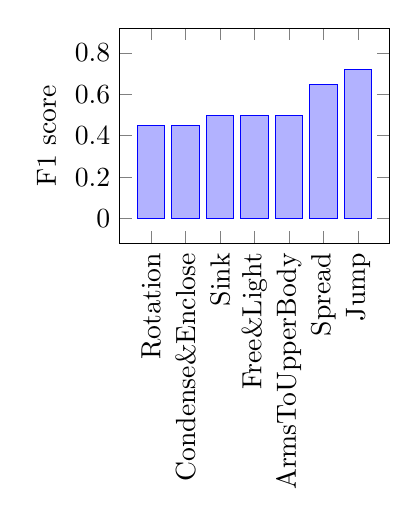
\begin{tikzpicture}
\begin{axis}[
    ymin=0,
    ymax=0.8,
    width=5cm,
    ybar stacked,
    enlargelimits=0.15,
    ylabel={F1 score},
    symbolic x coords={Rotation,Condense\&Enclose,Sink,Free\&Light,ArmsToUpperBody,Spread,Jump},
    xtick=data,
    x tick label style={rotate=90,anchor=east},
    ]
\addplot+[ybar] plot coordinates  {(Rotation,0.45) (Condense\&Enclose,0.45) (Sink,0.5) 
		(Free\&Light,0.5) (ArmsToUpperBody,0.5) (Spread, 0.65) (Jump,0.72)};

\end{axis}
\end{tikzpicture}
\caption{Performance on ordinary  people (non-CMAs) instructed to perform several tasks.}
\label{nonCMAs}
\end{figure}

\subsubsection{Evaluation performance for movements of unseen CMA}
In this experiment the test set was taken from the clips of one CMA while the
training set was composed from the clips of all other 5 CMAs. Testing was
performed for each CMA separately and the results were averaged over all six
CMAs. Performance as measured by F1 degraded on the unseen CMA from 0.6 to 0.57.
This degradation seems mild considering the large variation/diversity among
clips from one CMA to another, as every CMA performed different gestures, in
different postures (some sitting and some standing) and in different contexts
(some were dancing while some were acting).
\subsubsection{Evaluation performance for everyday movements of non-CMAs}
The data set of non-CMAs consisted of several daily movements two people were
asked to do, such as pretending to greet a friend or play with a balloon. This
data set was small, and the people were instructed to do movements that we hoped
would include the Laban motor elements that we have examined in this study, but
we had no direct control over the exact movement they chose to do or the motor
elements included in those movements. A CMA who watched those movements
determined which of the 18 Laban motor elements examined in this study appeared
in those movement sequences. As shown in Fig 5, which describes the learning
performance for this data set, it turned out that only 7 motor elements of the
18 examined in this study appeared in those people's movements. Performance as
measured by average F1 degraded from 0.57 for an unseen CMA to 0.54 for a
non-CMA.


\thesisbibfiles{bib}
\thesisbibstyle{alpha}